\documentclass[notitlepage,nofootinbib,showpacs,preprintnumbers,amsmath,amssymb,superscriptaddress,prd,onecolumn]{revtex4-1}
\pdfoutput=1
\usepackage{amsmath}
\usepackage[T1]{fontenc}
\usepackage{bm}
\usepackage{todonotes}
\usepackage[normalem]{ulem}
\usepackage{hyperref}
\usepackage{subcaption}
% \usepackage{showkeys}

\newcommand{\red}[1]{{\color{red} #1}}

\newcommand{\Neff}{\ensuremath{N_{\rm eff}}}
\newcommand{\DNeff}{\ensuremath{\Delta N_{\rm eff}}}
\newcommand{\dmsq}[1]{\ensuremath{\Delta m^2_{#1}}}
\newcommand{\uasq}[1]{\ensuremath{|U_{#1 4}|^2}}
\newcommand{\e}[1]{\ensuremath{\times10^{#1}}}

\newcommand{\fortepiano}{\texttt{FortEPiaNO}}
\newcommand{\dlsoda}{\texttt{DLSODA}}

\begin{document}
\title{\boldmath \fortepiano\ technical notes}

\author{S.\ Gariazzo}
\email{gariazzo@to.infn.it}
\affiliation{INFN, Sezione di Torino, Via P. Giuria 1, I--10125 Torino, Italy}

\author{P.F.\ de Salas}
\email{pablo.fernandez@fysik.su.se}
\affiliation{The Oskar Klein Centre for Cosmoparticle Physics,
Department of Physics, Stockholm University, SE-106 91 Stockholm, Sweden}

\author{S.\ Pastor}
\email{pastor@ific.uv.es}
\affiliation{Instituto de F{\'\i}sica Corpuscular  (CSIC-Universitat de Val{\`e}ncia), Valencia, Spain}


\maketitle


We present here the main features of
our code, \texttt{FORTran-Evolved PrimordIAl Neutrino Oscillations}
(\fortepiano) \cite{Gariazzo:2019gyi}.
The code is publicly available at the url
\url{https://bitbucket.org/ahep_cosmo/fortepiano_public}.


\section{Equations}
\fortepiano\ can compute oscillations with up to six neutrinos%
\footnote{The number six is hard-coded for implementation reasons, but it can be changed.}
in the early universe.
Neutrinos, including the sterile ones, are always treated as ultra-relativistic particles, which is a good approximation if the
neutrino masses do not exceed $\mathcal{O}(\mbox{a few keV})$,
i.e.\ neutrinos are still fully relativistic at decoupling.
For larger masses, neutrinos may start to become non-relativistic before decoupling,
and in that case one should take into account the effect of their mass.

The code computes the evolution of the
$N\times N$ neutrino density matrix
\cite{deSalas:2016ztq,Mirizzi:2012we,Saviano:2013ktj,Mangano:2001iu}
\begin{equation}\label{eq:varrho-B4}
\varrho(x, y)
=
\left(
\begin{array}{ccccc}
\varrho_{ee}&\varrho_{e\mu}&\varrho_{e\tau}&\varrho_{es_1}&\ldots\\
\varrho_{\mu e}&\varrho_{\mu\mu}&\varrho_{\mu\tau}&\varrho_{\mu s_1}&\\
\varrho_{\tau e}&\varrho_{\tau\mu}&\varrho_{\tau\tau}&\varrho_{\tau s_1}&\\
\varrho_{s_1e}&\varrho_{s_1\mu}&\varrho_{s_1\tau}&\varrho_{s_1s_1}&\\
\vdots&&&&\ddots
\end{array}
\right)\,,
\end{equation}
which is assumed to be the same for neutrinos and antineutrinos,
in terms of the comoving coordinates
$x\equiv m_e\, a$, $y\equiv p\, a$, $z\equiv T_\gamma\, a$ and $w\equiv T_\nu\,a$.
The momentum dependence of the density matrix $\varrho$ is taken into account
using a discrete grid of momenta, as described in section~\ref{ssec:momenta}.

The main goal of the code is to use the final value of $\varrho(x,y)$ to obtain
the effective number of relativistic degrees of freedom in the early Universe, \Neff.
Such number is well defined only before or after
the transition of electrons to the non-relativistic regime.
This means we have two possibilities:
\begin{itemize}
 \item at very early times, when neutrinos are completely coupled to the plasma and electrons are fully relativistic, neutrinos and photons share the same temperature and we have
\begin{equation}
\Neff^e
=
\frac{8}{7}
\frac{\sum_i \rho_{\nu_i}}{\rho_\gamma}
\qquad\text{at early times,}
\end{equation}
\item at late times, electrons become non-relativistic and their entropy is transfered to photons in the process.
Neutrinos are already partially decoupled, so that their energy density is not increased by the entropy transfer
and they end up with a smaller temperature than photons,
so that the new definition of \Neff\ is
\begin{equation}
\Neff^l
=
\frac{8}{7}
\left(\frac{11}{4}\right)^{4/3}
\frac{\sum_i \rho_{\nu_i}}{\rho_\gamma}
\qquad\text{at late times,}
\end{equation}
\end{itemize}
In both cases,
$\rho_\gamma$ is the comoving energy density of photons and
$\rho_{\nu_i}$ is the one of the $i$-th neutrino.

In order to write the evolution equations for the density matrix $\varrho$,
several quantities must be defined.
One of them is the neutrino mixing matrix,
of which we ignore the complex nature connected to the existence of CP violation
(the CP violating phase is set to zero).
When using $N$ neutrinos,
the mixing matrix is defined as
%
\begin{equation}\label{eq:mixing_matrix_nxn}
U=R^{(N-1)N} \ldots R^{1N}
R^{(N-2)(N-1)}\ldots R^{1(N-1)}
\ldots
R^{34} R^{24} R^{14} R^{23} R^{13} R^{12},
\end{equation}
%
following and extending the convention presented in Eq.~(12) of \cite{Gariazzo:2015rra},
where each $R^{ij}$ is a real rotation matrix described by the angle $\theta_{ij}$,
containing $\cos\theta_{ij}$ in the diagonal elements $ii$ and $jj$,
1 in the remaining diagonal elements,
$\sin\theta_{ij}$ ($-\sin\theta_{ij}$) in the off-diagonal element $ij$ ($ji$)
and zero otherwise:
\begin{equation}
\label{eq:rotationmatrix}
[R^{ij}]_{rs}=
\delta_{rs}
+
(\cos\theta_{ij}-1)(\delta_{ri}\delta_{si}+\delta_{rj}\delta_{sj})
+
\sin\theta_{ij}(\delta_{ri}\delta_{sj}-\delta_{rj}\delta_{si})\,.
\end{equation}
The neutrino mixing matrix enters the calculation of the rotated mass matrix
$\mathbb{M}_{\rm F}=U\mathbb{M}U^\dagger$,
where the diagonal mass matrix is
$\mathbb{M}=\text{diag}(m_1^2,\ldots,m_N^2)$.
Other matrices that we need to define are
%
\begin{equation}\label{eq:matterpotentials_nxn}
\mathbb{E}_\ell=\text{diag}(\rho_e, \rho_\mu, 0, \ldots)\,,
\qquad
\mathbb{P}_\ell=\text{diag}(P_e, P_\mu, 0, \ldots)\,,
\qquad
\mathbb{E}_\nu=S_a\frac{1}{\pi^2}\left(\int \mathrm{d}y y^3\varrho\right) S_a\,
\quad\mbox{with }S_a=\text{diag}(1,1,1,0,\ldots)\,,
\end{equation}
while the interaction matrices used in the the collision terms,
presented in section~\ref{sec:collint}, are
\begin{equation}
\label{eq:gLR}
G^L=\text{diag}(g_L, \tilde g_L, \tilde g_L, 0,\ldots)\,,
\qquad
G^R=\text{diag}(g_R, g_R, g_R, 0,\ldots)\,,
\end{equation}
%
where $g_L=\sin^2\theta_W+1/2$, $\tilde g_L=\sin^2\theta_W - 1/2$, $g_R=\sin^2\theta_W$,
and $\theta_W$ is the weak mixing angle.
Note that, in principle, one should use the values of $g_L$, $\tilde g_L$ and $g_R$
at zero momentum transfer \cite{Erler:2013xha},
instead of the ones obtained by measuring the weak mixing angle at the $Z$-pole.
Changing between the two possible sets of values (see section~\ref{ssec:precompiler})
does not alter the final result on \Neff\ by more than $10^{-4}$.

The definitions of comoving energy density and pressure,
which can be combined to obtain the comoving entropy density,
are written as:
\begin{eqnarray}
\rho_i
&=&
g_i
\int\frac{dp}{2\pi^2}\,
p^2 E_p \frac{1}{e^{E_p/z}\pm1}
\,,
\\
P
&=&
g_i
\int\frac{dp}{2\pi^2}\,
\frac{p^4}{3 E_p} \frac{1}{e^{E_p/z}\pm1}
\,,
\\
s
&=&
\frac{\rho+P}{z}
\,,
\end{eqnarray}
where the + (-) applies for fermions (bosons),
$i$ denotes the species, which has $g_i$ degrees of freedoms,
$p$ is the comoving momentum,
$E_p=\sqrt{p^2 + m_i^2}$, being $m_i$ the comoving mass of the particle,
and $z$ must be substituted with $w$ in the case of neutrinos.

To take into account finite temperature QED (FTQED) corrections
\cite{Fornengo:1997wa,Mangano:2001iu,Bennett:2019ewm},
we have to modify the total pressure and energy density of the fluid:
\begin{eqnarray}
P
&=&
\sum_{i=\gamma,{\nu_i},e,\mu}P_i
+
\delta P(x,z)
\,,\\
\rho
&=&
\sum_{i=\gamma,{\nu_i},e,\mu}\rho_i
+
\delta\rho(x,z)
\,,
\end{eqnarray}
where $\delta P$ and $\delta\rho$ are contributions that can be computed using FTQED.
It is convenient to define them
in terms of the following functions:
\begin{eqnarray}
J_a(r)
&=&
\frac{1}{\pi^2}
\int_0^\infty {\rm d}u \, u^a
\frac{\exp(\sqrt{u^2+r^2})}{\Big[\exp(\sqrt{u^2+r^2})+1\Big]^2}
\label{eq:j}
\,,\\
K_a(r)
&=&
\frac{1}{\pi^2}
\int_0^\infty {\rm d}u \, 
\frac{u^a}{\sqrt{u^2+r^2}}\,
\frac{1}{\exp(\sqrt{u^2+r^2})+1}
\label{eq:k}\,.
\end{eqnarray}
Let us also define for convenience:
\begin{eqnarray}
\mathcal{N}_p
&=&
\frac{2}{e^{E_p/z}+1}
\,,\\
\partial_x\mathcal{N}_p
&=&
-\frac{x\,e^{E_p/z}\,\mathcal{N}_p^2}{2z\,E_p}
\,,\\
\partial_z\mathcal{N}_p
&=&
\frac{
 e^{E_p/z}\,
 E_p\,
 \mathcal{N}_p^2
}{2 z^2}
\,,\\
\partial_x\partial_z\mathcal{N}_p
&=&
\frac{
 x\,
 e^{E_p/z}\,
 \mathcal{N}_p^2
}{2z^3}
\left(
 1
 -e^{E_p/z}\,\mathcal{N}_p
 +\frac{z}{E_p}
\right)
\,.
\end{eqnarray}
The contributions $\delta P$ and $\delta\rho$ can be expanded as a series of powers of the electron charge
$e^2=4\pi\alpha$, where $\alpha$ is the fine structure constant.
Taking into account the first orders of the expansion, and using $r=x/z$, for the pressure one has \cite{Bennett:2019ewm}
%
\begin{eqnarray}
\delta P(x,z)
&=&
\delta P^{(2)}(x/z)
+
\delta P^{(2+\ln)}(x,z)
+
\delta P^{(3)}(x/z)
+\ldots
\,,
\\
\delta P^{(2)}(r)
&=&
-
e^2 z^4\,K_2
\left(
 \frac{1}{6}
 +\frac{K_2}{2}
\right)
\,,\\
\delta P^{(2+\ln)}(x,z)
&=&
\frac{e^2 x^2}{16\pi^4}
\int\!\!\!\int_0^\infty
{\rm d}y\,
{\rm d}k\,
\frac{y\,k}{E_y E_k}
\ln
\left|
\frac{y+k}{y-k}
\right|
\mathcal{N}_y\,
\mathcal{N}_k
\,,\\
\delta P^{(3)}(r)
&=&
\frac{2e^3z^4}{3\pi}
\left(
K_2
+
\frac{r^2}{2} K_0
\right)^{3/2}
\,,
\end{eqnarray}
while for the energy density the various terms are
\begin{eqnarray}
\delta\rho(x,z)
&=&
\delta\rho^{(2)}(x/z)
+
\delta\rho^{(2+\ln)}(x,z)
+
\delta\rho^{(3)}(x/z)
+\ldots
\,,
\\
\delta\rho^{(2)}(r)
&=&
e^2 z^4
\left(
\frac{K_2^2}{2}
-\frac{K_2+J_2}{6}
-K_2 J_2
\right)
\,,\\
\delta\rho^{(2+\ln)}(x,z)
&=&
\frac{e^2 x^2}{16\pi^4}
\int\!\!\!\int_0^\infty
{\rm d}y\,
{\rm d}k\,
\frac{y\,k}{E_y E_k}
\ln
\left|
\frac{y+k}{y-k}
\right|
\mathcal{N}_y
\Big(
2z \partial_z \mathcal{N}_k
- \mathcal{N}_k
\Big)
\,,\\
\delta\rho^{(3)}(r)
&=&
\frac{e^3z^4}{\pi}
\left(
K_2
+
\frac{r^2}{2} K_0
\right)^{1/2}
\left(
J_2
+
\frac{r^2}{2} J_0
\right)
\,.
\end{eqnarray}

In order to compute the evolution of the neutrino density matrix \eqref{eq:varrho-B4},
we have to compute both the derivative of $\varrho$ (as a function of the momentum)
and of the comoving photon temperature $z$
with respect to our time parameter $x$.
The differential equations which the code solves are the following
\cite{deSalas:2016ztq,Mirizzi:2012we,Saviano:2013ktj,Mangano:2001iu}:
%
\begin{eqnarray}\label{eq:drho_dx_nxn}
\frac{{\rm d}\varrho(y)}{{\rm d}x}
&=&
\sqrt{\frac{3 m^2_{\rm Pl}}{8\pi\rho}}
\left\{
    -i \frac{x^2}{m_e^3}
    \left[
        \frac{\mathbb{M}_{\rm F}}{2y}
        -
        \frac{2\sqrt{2}G_{\rm F} y m_e^6}{x^6}
        \left(
            \frac{\mathbb{E}_\ell+\mathbb{P}_\ell}{m_W^2}
            +
            \frac{4}{3}\,\frac{\mathbb{E}_\nu}{m_Z^2}
        \right),
    \varrho
    \right]
    +\frac{m_e^3}{x^4}\mathcal{I(\varrho)}
\right\}\,,
\nonumber\\
\label{eq:dz_dx_nxn}
\frac{\mathrm{d}z}{\mathrm{d}x}
&=&
\cfrac{
{\displaystyle \sum_{\ell=e,\mu}}
\left[
\cfrac{r_\ell^2}{r} J_2(r_\ell)
\right]
+ G_1(r)
- \cfrac{1}{2\pi^2z^3}
    {\displaystyle \int_0^\infty \mathrm{d}y\,y^3\sum_{\alpha=e}^{s_{N_s}^{}}\cfrac{\mathrm{d}\varrho_{\alpha \alpha}}{\mathrm{d}x}}
}{
{\displaystyle \sum_{\ell=e,\mu}}
\Big[
r^2_\ell J_2(r_\ell)
+ J_4(r_\ell)
\Big]
+ G_2(r)
+ \cfrac{2\pi^2}{15}
}\,,
\end{eqnarray}
where $r_\ell=m_\ell/m_e\,r$.
The expressions for the $G_1$ and $G_2$ functions,
which again take into account the FTQED corrections, are written as
\cite{Mangano:2001iu,Bennett:2019ewm}:
%
\begin{eqnarray}
G_{1,2}(x,z)
&=&
G_{1,2}^{(2)}(x/z)
+
G_{1,2}^{(2+\ln)}(x,z)
+
G_{1,2}^{(3)}(x/z)
+
\ldots
\,,
\end{eqnarray}
%
\begin{eqnarray}
G_a(r)
&=&
\frac{K_2'}{6}
-K_2K_2'
+\frac{J_2'}{6}
+K_2'J_2
+K_2J_2'
\,,\\
G_1^{(2)}(r)
&=&
2\pi\alpha
\left[
  \frac{1}{r}
  \left(
    \frac{K_2}{3}
    + 2 K_2^2
    -\frac{J_2}{6}
    -K_2J_2
  \right)
  +
  G_a
\right]
\label{eq:g1}
\,,\\
G_2^{(2)}(r)
&=&
-8\pi\alpha
\left(
  \frac{K_2}{6}
  +\frac{J_2}{6}
  -\frac{1}{2}K_2^2
  +K_2J_2
\right)
+
2\pi\alpha r
G_a
\label{eq:g2}
\,,
\end{eqnarray}
%
\begin{eqnarray}
G_1^{(2+\ln)}(x,z)
&=&
\frac{e^2 x}{16\pi^4 z^3}
\int\!\!\!\int_0^\infty
{\rm d}y\,
{\rm d}k\,
\frac{y\,k}{E_y E_k}
\ln\left|\frac{y+k}{y-k}\right|
\Bigg\{
-x\bigg[
  z\Big(
    \partial_x\mathcal{N}_y\partial_z\mathcal{N}_k
    +
    \mathcal{N}_y\partial_x\partial_z\mathcal{N}_k
  \Big)
  -\mathcal{N}_y\partial_x\mathcal{N}_k
\bigg]
\nonumber\\
&&
\qquad\qquad\qquad\qquad
-\mathcal{N}_y\mathcal{N}_k
-z\mathcal{N}_y\partial_z\mathcal{N}_k
+\frac{x^2 (E_y^2+E_k^2)}{2 E_y^2 E_k^2}
\Big(
2z \mathcal{N}_y\partial_z \mathcal{N}_k
-\mathcal{N}_y \mathcal{N}_k
\Big)
\Bigg\}
\,,\\
G_2^{(2+\ln)}(x,z)
&=&
\frac{e^2 x^2}{16\pi^4 z^2}
\int\!\!\!\int_0^\infty
{\rm d}y\,
{\rm d}k\,
\frac{y\,k}{E_y E_k}
\ln\left|\frac{y+k}{y-k}\right|
\partial_z
\Big(
\mathcal{N}_y
\partial_z
\mathcal{N}_k
\Big)
\,,
\end{eqnarray}
%
\begin{eqnarray}
G_b(r)
&=&
\sqrt{K_2 + r^2 \frac{K_0}{2}}
\,,\\
G_c(r)
&=&
\frac{2J_2 + r^2 J_0}{2\Big(2K_2 + r^2 K_0\Big)}
\,,\\
G_1^{(3)}(r)
&=&
\frac{e^3}{4\pi} G_b
\left\{
 \frac{1}{r}\Big(2J_2-4K_2\Big)
 -2J_2'
 -r^2J_0'
 -r\Big(2K_0+J_0\Big)
 -G_c\Big[r(K_0-J_0)+K_2'\Big]
\right\}
\,,\\
G_2^{(3)}(r)
&=&
\frac{e^3}{4\pi} G_b
\left[
 G_c \Big(2J_2 + r^2 J_0\Big)
 -\frac{2}{r}J_4'
 -r\Big(3J_2'+r^2J_0'\Big)
\right]
\,,
\label{eq:g3}
\end{eqnarray}
%
where the prime denotes derivative with respect to $r$ and we dropped the explicit dependence on $r$ in the expressions for the $G$ functions.
For the sake of computational speed, the code can calculate and store lists for all the terms of Eq.~\eqref{eq:dz_dx_nxn}
which do not depend on the neutrino density matrix 
at the initialisation stage, and compute their values through interpolation during the real calculation.
The same happens for the energy densities of charged leptons, for which performing an interpolation
is much faster than computing an integral.
The interpolation, however, can be disabled during compilation (see section~\ref{ssec:precompiler}),
with a $\lesssim20$\% increase of the running time.

The finite-temperature electromagnetic corrections are also taken into account in the calculation
of the electron mass, used in the collision terms, discussed in the following section.
The additional contribution to the electron mass, in comoving coordinates, is obtained as \cite{Fornengo:1997wa,Mangano:2001iu,Bennett:2019ewm}:
\begin{equation}
\delta m_e^2(x, y, z)
=
\frac{2\pi\alpha z^2}{3}
+
\frac{4\alpha}{\pi}
\int_0^\infty{\rm d}k\,
\frac{k^2}{E_k}
\frac{1}{e^{E_k/z}+1}
-
\frac{x^2\alpha}{\pi y}
\int_0^\infty{\rm d}k\,
\frac{k}{E_k}
\log\left|\frac{y+k}{y-k}\right|
\mathcal{N}_k
\,,
\end{equation}
so that the comoving electron mass must be replaced using $x^2\rightarrow x^2+\delta m_e^2$.
In the calculation of the collision integrals we ignore the log term that depends on $y$.

Finally, in order to estimate the effective comoving neutrino temperature $w$, which is
not needed for the calculation but useful to understand the final results,
we use an equation similar to Eq.~\eqref{eq:dz_dx_nxn},
but considering only relativistic electrons, i.e.\ fixing $r_e=0$ in the equation.


\section{Collision integrals}
\label{sec:collint}
The full collision terms are defined by the sum
of the contributions from neutrino--electron/positron scattering and
$e^\pm$ annihilation into neutrinos,
plus neutrino--neutrino interactions.
We neglect other reactions, such as $\mu^\pm$ annihilation (which only affects at very early temperatures when everything is in equilibrium).
We therefore have \cite{deSalas:2016ztq,Bennett:2020zkv}
%
\begin{eqnarray}
\mathcal{I}[\varrho(y)]
&=&
\frac{G_F^2}{(2\pi)^3y^2}
\mathcal{I}^u\,,
\label{eq:collint}
\\
\mathcal{I}^u
&\equiv&
\mathcal{I}_{\rm sc}^u
+ \mathcal{I}_{\rm ann}^u
+ \mathcal{I}_{\nu\nu}^u
+ \mathcal{I}_{\nu\bar\nu}^u
\,,
\label{eq:unnormcollint}
\\
\mathcal{I}_{\rm sc} ^u
&=&
\int {\rm d}y_2 {\rm d}y_3 \frac{y_2}{E_2} \frac{y_4}{E_4}
\label{eq:I_sc}
\\
&&
\left\{\left(\Pi_2^s(y, y_4)+\Pi_2^s(y, y_2)\right)
    \left[
    F_{\rm sc}^{LL}\left(\varrho^{(1)}, f_e^{(2)}, \varrho^{(3)}, f_e^{(4)}\right)
    +F_{\rm sc}^{RR}\left(\varrho^{(1)}, f_e^{(2)}, \varrho^{(3)}, f_e^{(4)}\right)\right]\right.
    \nonumber\\
    &&\left.-2(x^2+\delta m_e^2)\Pi_1^s(y,y_3)
    \left[
     F_{\rm sc}^{RL}\left(\varrho^{(1)}, f_e^{(2)}, \varrho^{(3)}, f_e^{(4)}\right)
    +F_{\rm sc}^{LR}\left(\varrho^{(1)}, f_e^{(2)}, \varrho^{(3)}, f_e^{(4)}\right)
    \right]\nonumber
\right\}\,,
\\
\mathcal{I}_{\rm ann}^u
&=&
\int {\rm d}y_2 {\rm d}y_4 \frac{y_3}{E_3} \frac{y_4}{E_4}
\label{eq:I_ann}\\
    &&\left\{\Pi_2^a(y, y_4)F_{\rm ann}^{LL}\left(\varrho^{(1)}, \varrho^{(2)}, f_e^{(3)}, f_e^{(4)}\right)
    +\Pi_2^a(y, y_3)F_{\rm ann}^{RR}\left(\varrho^{(1)}, \varrho^{(2)}, f_e^{(3)}, f_e^{(4)}\right)\right.
\nonumber\\
    &&\left.+ (x^2+\delta m_e^2)\Pi_1^a(y,y_2)
    \left[
    F_{\rm ann}^{RL}\left(\varrho^{(1)}, \varrho^{(2)}, f_e^{(3)}, f_e^{(4)}\right)
    +F_{\rm ann}^{LR}\left(\varrho^{(1)}, \varrho^{(2)}, f_e^{(3)}, f_{e^+}^{(4)}\right)
    \right]\nonumber
\right\}\,,
\\
\mathcal{I}_{\nu\nu} ^u
&=&
\frac{1}{4}
\int {\rm d}y_2 {\rm d}y_3\,
\Pi_2^\nu(y, y_2)
F_{\nu\nu}\left(\varrho^{(1)}, \varrho^{(2)}, \varrho^{(3)}, \varrho^{(4)}\right)
\,,
\label{eq:I_nunu}
\\
\mathcal{I}_{\nu\bar\nu} ^u
&=&
\frac{1}{4}
\int {\rm d}y_2 {\rm d}y_3\,
\Pi_2^\nu(y, y_4)
F_{\nu\bar\nu}\left(\varrho^{(1)}, \varrho^{(2)}, \varrho^{(3)}, \varrho^{(4)}\right)
% F_{\nu\bar\nu}\left(\varrho^{(1)}, \bar\varrho^{(2)}, \varrho^{(3)}, \bar\varrho^{(4)}\right)
\label{eq:I_nubarnu}
\,,
\end{eqnarray}
where $E^2_i = \sqrt{x^2+y_i^2+\delta m_e^2}$ and
\begin{eqnarray}
\Pi_1^s(y,y_3)
&=&
y\,y_3\,D_1+D_2(y,y_3,y_2,y_4),
\\
\Pi_1^a(y,y_2)
&=&
y\,y_2\,D_1-D_2(y,y_2,y_3,y_4),
\\
\Pi_2^s(y,y_2)/2
&=&
y\,E_2\,y_3\,E_4\,D_1 + D_3 - y\,E_2 D_2(y_3,y_4,y,y_2) - y_3\,E_4 D_2(y,y_2,y_3,y_4),
\\
\Pi_2^s(y,y_4)/2
&=&
y\,E_2\,y_3\,E_4\,D_1 + D_3 + E_2\,y_3 D_2(y,y_4,y_2,y_3) + y\,E_4 D_2(y_2,y_3,y,y_4),
\\
\Pi_2^a(y,y_3)/2
&=&
y\,y_2\,E_3\,E_4\,D_1 + D_3 + y\,E_3 D_2(y_2,y_4,y,y_3) + y_2\,E_4 D_2(y,y_3,y_2,y_4),
\\
\Pi_2^a(y,y_4)/2
&=&
y\,y_2\,E_3\,E_4\,D_1 + D_3 + y_2\,E_3 D_2(y,y_4,y_2,y_3) + y\,E_4 D_2(y_2,y_3,y,y_4),
\\
\Pi_2^\nu(y,y_2)/2
&=&
y\,y_2\,y_3\,y_4\,D_1 + D_3 - y\,y_2 D_2(y_3,y_4,y,y_2) - y_3\,y_4 D_2(y,y_2,y_3,y_4),
\\
\Pi_2^\nu(y,y_4)/2
&=&
y\,y_2\,y_3\,y_4\,D_1 + D_3 + y_2\,y_3 D_2(y,y_4,y_2,y_3) + y\,y_4 D_2(y_2,y_3,y,y_4),
\end{eqnarray}
%
where the functions $D_i$ have the following definitions \cite{Dolgov:1997mb}:
%
\begin{eqnarray}
D_1(a,b,c,d)
&=&
\frac{16}{\pi}
\int_0^\infty
\frac{{\rm d}\lambda}{\lambda^2}
\prod_{i=a,b,c,d}\sin(\lambda i)
\,,\\
D_2(a,b,c,d)
&=&
-\frac{16}{\pi}
\int_0^\infty
\frac{{\rm d}\lambda}{\lambda^4}
\prod_{i=a,b}\Big[\lambda i \cos(\lambda i)-\sin(\lambda i)\Big]
\prod_{j=c,d}\sin(\lambda j)
\,,\\
D_3(a,b,c,d)
&=&
\frac{16}{\pi}
\int_0^\infty
\frac{\mathrm{d}\lambda}{\lambda^6}
\prod_{i=a,b,c,d}\Big[\lambda i \cos(\lambda i)-\sin(\lambda i)\Big]
\,.
\end{eqnarray}
These three integrals can be solved analytically,
and therefore the three functions $D_{1, 2, 3}$ can be coded in a more efficient way,
not reported here for sake of brevity
(see e.g.~\cite{Blaschke:2016xxt}).

Finally, the functions that define the phase space factors in the collision terms are \cite{deSalas:2016ztq,Bennett:2020zkv}:
\begin{eqnarray}
F_{\rm sc}^{ab}\left(\varrho^{(1)}, f_e^{(2)}, \varrho^{(3)}, f_e^{(4)}\right)
&=&
f_e^{(4)}(1-f_e^{(2)})\left[G^a\varrho^{(3)}G^b(1-\varrho^{(1)})+(1-\varrho^{(1)})G^b\varrho^{(3)}G^a\right]
\nonumber\\
&-&
f_e^{(2)}(1-f_e^{(4)})\left[\varrho^{(1)}G^b(1-\varrho^{(3)})G^a+G^a(1-\varrho^{(3)})G^b\varrho^{(1)}\right],
\label{eq:F_ab_sc}\\
F_{\rm ann}^{ab}\left(\varrho^{(1)}, \varrho^{(2)}, f_e^{(3)}, f_e^{(4)}\right)
&=&
f_e^{(3)}f_e^{(4)}\left[G^a(1-\varrho^{(2)})G^b(1-\varrho^{(1)})+(1-\varrho^{(1)})G^b(1-\varrho^{(2)})G^a\right]
\nonumber\\
&-&
(1-f_e^{(3)})(1-f_e^{(4)})\left[G^a\varrho^{(2)}G^b\varrho^{(1)}+\varrho^{(1)}G^b\varrho^{(2)}G^a\right],
\label{eq:F_ab_ann}
\\
F_{\nu\nu}\left(\varrho^{(1)}, \varrho^{(2)}, \varrho^{(3)}, \varrho^{(4)}\right)
&=&
\left(1-\varrho^{(1)}\right)\varrho^{(3)}
\left[\left(1-\varrho^{(2)}\right)\varrho^{(4)}+\mathrm{Tr}(\cdots)\right]
\nonumber\\
&-&
\varrho^{(1)}\left(1-\varrho^{(3)}\right)
\left[\varrho^{(2)}\left(1-\varrho^{(4)}\right)+\mathrm{Tr}(\cdots)\right]
+\mathrm{h.c.}
\label{eq:F_nunu}\\
F_{\nu\bar\nu}\left(\varrho^{(1)}, \varrho^{(2)}, \varrho^{(3)}, \varrho^{(4)}\right)
&=&
\left(1-\varrho^{(1)}\right)\left(1-\varrho^{(2)}\right)
\left[\varrho^{(4)}\varrho^{(3)}+\mathrm{Tr}(\cdots)\right]
\nonumber\\
&-&
\varrho^{(1)}\varrho^{(2)}
\left[\left(1-\varrho^{(4)}\right)\left(1-\varrho^{(3)}\right)+\mathrm{Tr}(\cdots)\right]
\nonumber\\
&+&
\left(1-\varrho^{(1)}\right)\varrho^{(3)}
\left[\varrho^{(4)}\left(1-\varrho^{(2)}\right)+\mathrm{Tr}(\cdots)\right]
\nonumber\\
&-&
\varrho^{(1)}\left(1-\varrho^{(3)}\right)
\left[\left(1-\varrho^{(4)}\right)\varrho^{(2)}+\mathrm{Tr}(\cdots)\right]
% F_{\nu\bar\nu}\left(\varrho^{(1)}, \bar\varrho^{(2)}, \varrho^{(3)}, \bar\varrho^{(4)}\right)
% &=&
% \left(1-\varrho^{(1)}\right)\left(1-\bar\varrho^{(2)}\right)
% \left[\bar\varrho^{(4)}\varrho^{(3)}+\mathrm{Tr}(\cdots)\right]
% \nonumber\\
% &-&
% \varrho^{(1)}\bar\varrho^{(2)}
% \left[\left(1-\bar\varrho^{(4)}\right)\left(1-\varrho^{(3)}\right)+\mathrm{Tr}(\cdots)\right]
% \nonumber\\
% &+&
% \left(1-\varrho^{(1)}\right)\varrho^{(3)}
% \left[\bar\varrho^{(4)}\left(1-\bar\varrho^{(2)}\right)+\mathrm{Tr}(\cdots)\right]
% \nonumber\\
% &-&
% \varrho^{(1)}\left(1-\varrho^{(3)}\right)
% \left[\left(1-\bar\varrho^{(4)}\right)\bar\varrho^{(2)}+\mathrm{Tr}(\cdots)\right]
+\mathrm{h.c.},
\label{eq:F_nubarnu}
\end{eqnarray}
where $\varrho^{(i)}=\varrho(y_i)$ and $f_e^{(i)}=f_{\rm FD}(y_i, z)$ represent the momentum distribution function
of the various particles,
and $\mathrm{Tr}(\cdots)$ denotes the trace of the term immediately before it.
The full expression for these functions should take into account the lepton asymmetry and distinguish
the momentum distributions of leptons/neutrinos from those of antilepton/antineutrinos.
Since we do not include lepton asymmetry, we just report the expressions without the heavier notation
required to distinguish the contribution of antiparticles.

Concerning the neutrino--neutrino collision terms \cite{Bennett:2020zkv},
there are few more points to be discussed.
We can see from Eqs.~\eqref{eq:F_nunu}--\eqref{eq:F_nubarnu} that the expressions include
up to four products of the neutrino density matrices at different momentum modes.
With a smart implementation of the integration methods
(see sections~\ref{ssec:momenta} and \ref{ssec:integrals}),
one can use for three of the terms (namely, the ones containing $y_1$, $y_2$ and $y_3$)
the values obtained on the momentum grid.
For the fourth occurrence, $\varrho(y_4)$, an interpolation is needed.
We tested several possibilities, and implemented a scheme that computes
the linear interpolation of $\varrho_{\alpha\alpha}/f_{\rm FD}$ on the diagonal,
and the linear interpolation of $\varrho_{\alpha\beta}$ ($\alpha\neq\beta$) for the off-diagonal,
as it guarantees a better numerical stability (see \cite{Bennett:2020zkv}).
Nevertheless, the selection of the momentum grid may have a strong impact on the results obtained using
neutrino--neutrino collision terms, as we will discuss in section~\ref{ssec:precision}.
We have also verified that the numerical values of \Neff\ obtained including the integrals in
Eqs.~\eqref{eq:I_nunu}--\eqref{eq:I_nubarnu}
does not vary significantly if we consider only the diagonal components of $\varrho$,
or we instead consider the full matrix.
The reason is that the off-diagonal terms are typically much smaller than the diagonal ones,
so that their combinations are suppressed and give a small contribution to the collision terms.
Ignoring the off-diagonal terms, therefore, gives a very precise result with a slightly smaller computational cost.
Notice also that the implementation of the neutrino--neutrino collision terms as described here
allows to compute off-diagonal collision terms
taking into account the full neutrino density matrix \cite{Bennett:2020zkv}.


\subsection*{Damping approximation}
The code can compute the collision terms according to Eqs.~\eqref{eq:I_sc}--\eqref{eq:I_nubarnu},
but the integrals are very expensive.
For the non-diagonal terms of the collision matrix we therefore allow the possibility to use
damping approximations, in the form
%
\begin{equation}
\mathcal{I}^u_{\alpha\beta}(\varrho) = -D^u_{\alpha\beta} \varrho_{\alpha\beta},
\end{equation}
%
for $\alpha \neq \beta$.
Notice that $\mathcal{I}^u_{\alpha\beta}(\varrho)$ is the unnormalized term
defined in Eq.~\eqref{eq:unnormcollint}.
The expressions for the coefficients $D^u_{\alpha\beta}$ depend on the elements considered.
In case more than one sterile state is considered, the terms $D^u_{s_is_j}$ are always zero.
For the rest of the terms, two possibilities are implemented in the code.

\paragraph{}
The first possibility arises from the calculations presented in the Appendix~B of \cite{Bennett:2020zkv}.
Notice that the appendix proposes also a damping approximation for diagonal collision terms,
which however is not implemented in \fortepiano.
According to \cite{Bennett:2020zkv}, we have a contribution from neutrino--neutrino interactions
that is flavour-blind (as expected, since in equilibrium there are the same number of neutrinos
and antineutrinos of each flavour), and one from neutrino--electron collisions.
We can write the damping terms in the following forms:
\begin{eqnarray}
\big\{D^u(y) \big\}_{\alpha \beta}
&=&
\frac{1}{2} \left[\big\{R^u(y) \big\}_\alpha+ \big\{R^u(y) \big\}_\beta \right],
\label{eq:damping_d_r}
\\
%nunu
\big\{R^u_{\nu \nu}(y) \big\}_{\alpha}
&=&
2
\int {\rm d}y_2 {\rm d}y_3 \,
\left[\Pi_{2}^{\nu}(y, y_2) + 2 \Pi_{2}^{\nu}(y, y_4) \right]
\nonumber\\
&&
\qquad
\times
\Big(
[1-f_{\rm eq}(y_2)] f_{\rm eq}(y_3) f_{\rm eq}(y_4)
+f_{\rm eq}(y_2) [1-f_{\rm eq}(y_3)][1-f_{\rm eq}(y_4)]
\Big)
\nonumber\\
&\equiv&
{\cal D}^u(y,z),
\label{eq:selfdamping}
\\
%nue
\{R^u_{\nu e}(y)\}_{\alpha}
&=&
\frac{1}{2} \,
\left[(2 \sin^2 \theta_W \pm 1)^2_\alpha + 4 \sin^4 \theta_W\right]
\int {\rm d}y_2 {\rm d}y_3 \,
\left[\Pi_{2}^{\nu}(y, y_2) + 2 \Pi_{2}^{\nu}(y, y_4) \right]
\nonumber\\
&&
\qquad
\times
\Big(
[1-f_{\rm eq}(y_2)] f_{\rm eq}(y_3) f_{\rm eq}(y_4)
+f_{\rm eq}(y_2) [1-f_{\rm eq}(y_3)][1-f_{\rm eq}(y_4)]
\Big)
\nonumber \\
&=&
\frac{1}{4}
\left[(2 \sin^2 \theta_W \pm 1)^2_\alpha + 4 \sin^4 \theta_W\right] {\cal D}^u(y,z),
\label{eq:nuedampingdiag}
\end{eqnarray}
where in the prefactor $(2 \sin^2 \theta_W\pm 1)_\alpha$  the plus sign ``$+$'' is understood to apply to $\alpha =e$ and ``$-$'' to $\alpha = \mu, \tau$.

For relativistic Fermi--Dirac distributions, the function ${\cal D}^u(y,z)$ evaluates to
\begin{equation}
{\cal D}^u(y,z) = 2 y^3 z^4 d(y/z)\,,
\label{eq:dy}
\end{equation}
where $d(s)$ is a number around 100 which can be obtained as a double momentum integral,
see Eq.~(B.9) in \cite{Bennett:2020zkv}.
For computational ease,
$d(s)$ can be fitted in the interval $s \in [10^{-4},10^3]$ to better than 0.25\% accuracy by the curve
\begin{equation}
d_{\rm fit}(s)
=
d_0 e^{-1.01 s}
+
d_\infty (1- e^{-0.01 s})
+
(e^{-0.01 s}-e^{-1.01 s})
\left[
\frac{a_0 + a_1 \ln  (s) + a_2 \ln^2(s)}{1 + b_1 \ln  (s) + b_2 \ln^2(s)}
\right]\,,
\label{eq:fittingfunctiondy}
\end{equation}
where $d_0 = 129.875$ and $d_\infty = 100.999$ are the asymptotic values of the function as $s \to 0$ and
$s \to \infty$ respectively, and the fitting coefficients are
$a_0 = 90.7332$, $a_1 = -48.4473$, $a_2 =20.1219$,
$b_1 = -0.529157$, and $b_2 = 0.20649$ \cite{Bennett:2020zkv}.



\paragraph{}
The second possibility is to implement the coefficients derived in \cite{McKellar:1992ja},
see also \cite{Enqvist:1991qj,Bell:1998ds},
under the assumption
\begin{equation}
\varrho(y)
=
\frac{
f_{\rm eq}(y)
}{
f_{\rm eq}(\langle y\rangle)
}
\varrho(\langle y\rangle)\,,
\end{equation}
such that (y) at all modes y evolve in phase,
where $\langle y\rangle$ denotes a representative momentum.
Upon integration in $y$,
the procedure yields a thermally-averaged collision term,
which can be written in the form
%
\begin{eqnarray}
D^u_{e\mu}/F=D^u_{e\tau}/F & = & 15 + 8\sin^4\theta_W\,,\\
D^u_{\mu\tau}/F & = & 7 - 4\sin^2\theta_W + 8\sin^4\theta_W\,,\\
D^u_{es}/F & = & 29 + 12\sin^2\theta_W + 24\sin^4\theta_W\,,\\
D^u_{\mu s}/F = D^u_{\tau s}/F & = & 29 - 12\sin^2\theta_W + 24\sin^4\theta_W\,,
\end{eqnarray}
where
$F=7\pi^4 z^4 y^3/135$ is a common normalisation coefficient.


\section{Solver and initial conditions}
\label{ssec:solver}
We solve the differential equations with the \dlsoda\ routine
from the \texttt{ODEPACK}%
\footnote{\url{https://computation.llnl.gov/casc/odepack/odepack_home.html}.}\
Fortran package \cite{hindmarsh1982odepack,dlsoda1}.
\texttt{ODEPACK} is a collection of solvers for the initial value problem for systems of ordinary differential equations.
It includes methods to deal with stiff and non-stiff systems, and some of the provided subroutines
automatically recognise which type of problem they are facing.

The specific solver we use, \dlsoda,
is a modification of the Double-precision Livermore Solver for Ordinary Differential Equations (\texttt{DLSODE})
which includes an automatic switching between stiff and non-stiff problems
of the form ${\rm d}y/{\rm d}t = f(t,y)$.
In the stiff case, it treats the Jacobian matrix ${\rm d}f/{\rm d}y$ as either a dense (full) or a banded matrix, and as either user-supplied or internally approximated by difference quotients.
It uses Adams methods (predictor--corrector) in the non-stiff case, and Backward Differentiation Formula (BDF) methods (the Gear methods) in the stiff case.
The linear systems that arise are solved by direct methods (LU factor/solve).
For more details, see the original publications  \cite{hindmarsh1982odepack,dlsoda1}.

The initial conditions for \dlsoda\ are defined as follows.
The initial time $x_{\rm in}$ is an input parameter of the code,
and reasonable values would correspond to temperatures between a few hundreds and a few tens of MeV.
The initial comoving photon temperature is computed evolving Eq.~\eqref{eq:dz_dx_nxn}
from even earlier times ($z_0=1$ at $T_0=10\, m_\mu$, $x_0=m_e/T_0$) until $x_{\rm in}$.
The obtained value $z_{\rm in}$ is then considered as the temperature of equilibrium
of the entire plasma. Concerning the neutrino density matrix at $x_{\rm in}$, all off-diagonal elements and the diagonal ones for sterile
neutrinos are fixed to zero, while the diagonal elements corresponding to active neutrinos are 
Fermi--Dirac distributions with a temperature $z_{\rm in}$.
For typical values that we use in the code,
we have $z_{\rm in}-1=2.9\e{-4}$ for $x_{\rm in}=0.001$ (which we use for the 3+1 cases)
or
$z_{\rm in} = 1.098$%
\footnote{
This number comes from our choice of normalisation of $z$ and the fact that
we take into account the presence of muons at high temperatures.
When muons become non-relativistic, they transfer their entropy to the rest of the plasma,
with the result that the photon temperature grows by a factor
$(57/43)^{1/3}\simeq 1.098$.
}
for $x_{\rm in}=0.05$ (suitable for the three-neutrino case, see \cite{deSalas:2016ztq}).
We verified \cite{Bennett:2020zkv} that the results on \Neff\ are not significantly affected by the choice of $x_{\rm in}$,
given that the initial temperature is sufficiently higher than the neutrino decoupling temperature.
Variations in the range $0.001\leq x_{\rm in}\leq 0.05$ generate differences in \Neff\ smaller
than $\sim2\times 10^{-5}$.


\section{Momentum grid}
\label{ssec:momenta}
In order to follow the evolution of Eq.~\eqref{eq:varrho-B4}, we discretise its dependence on $y$ and evolve each of the momentum in $x$.
One of the most interesting ways to make the code more precise and faster is related to the choice of the $y_i$.
First of all, we note that a logarithmic spacing of the $y_i$
will introduce biases in the numerical calculation
and that the final numbers of
the neutrino energy density and effective number may be artificially increased.
Inspired by one of the methods used in \texttt{CLASS} (see \cite{Lesgourgues:2011rh}),
we tested a spacing based on the Gauss--Laguerre (GL) integration method.
The crucial point of the calculation is to compute the energy density of neutrinos,
given by
%
\begin{equation}
\rho_\alpha
=
\frac{1}{\pi^2}
\int_0^\infty
\mathrm{d}y\, y^3\,\varrho_{\alpha\alpha}(y),
\end{equation}
%
where $\varrho_{\alpha\alpha}(y)$ will be close to a Fermi--Dirac distribution and in any case always exponentially suppressed.
The Gauss--Laguerre quadrature (see e.g.~\cite{NR})
is a method that is designed to optimise the solution of integrals of the type
\begin{equation}
I
=
\int_0^\infty
{\rm d}x\, y^\alpha\,e^{-y}\,f(y)
\simeq\sum_i^{N}w_i^{(\alpha)}\,f(y_i)
\,,
\end{equation}
where $f(y)$ is a generic function,
$y_i$ are the $N$ roots of the Laguerre polynomial $L_N$ of order $N$, and $w_i$ are relative weights,
which are obtained using
\begin{equation}
w_i^{(\alpha)}=
\frac{y_i}{\left(N+1\right)^2\left[L^{(\alpha)}_{N+1}(y_i)\right]^2}.
\end{equation}
The weights can be computed for example using the \texttt{gaulag} routine from \cite{NR}.
Since our momentum distribution function is not directly proportional to $e^{-y}$,
we consider $f(x)=e^y\,\varrho_{\alpha\alpha}(y)$,
in order to rescale the weights appropriately.

For the simple purpose of integrating the Fermi--Dirac distribution, very few points are typically required.
\texttt{CLASS}, for example, uses order of ten points for integrating the neutrino distribution function.
In our case, the non-thermal distortions must be computed accurately, and in particular
when evolving the thermalisation of a sterile neutrino we need more precision on the small momenta.
On the other hand, we do not want to compute the momentum distribution function at very high $y$,
which gives a very small contribution to the total integral.
We therefore use a truncated list of nodes $y_i$ over which to compute the evolution of $\varrho$,
selecting only the $N_y\leq N$ nodes for which $y_i<y_{\rm max}$.
In this way we can increase the number of points at small $y$ and the resolution on the thermalisation processes
without having to compute a large number of points at high momentum.
The number of points we can use is limited by the accuracy of the algorithm that computes the $w_i$.
For the \texttt{gaulag} routine \cite{NR}, our setup allows to reach $N_y\sim50$ when $N\sim350$,
when $y_i<y_{\rm max}=20$.
This number of momentum nodes
if neutrino--neutrino collision terms are ignored,
is already large enough to reach a precision
much better than one per mille on \Neff,
which is the same we could obtain with a linear spacing of the points
and $N_y=100$ \cite{deSalas:2016ztq}.
Since the evaluation of the collision integrals scales as $N_y^2$
and the number of derivatives in Eq.~\eqref{eq:drho_dx_nxn} scales with $N_y$,
this ensures a significant gain.
Unfortunately, since the method used to compute the GL nodes does not allow to increase $N_y$ arbitrarily,
the GL method has limitations when the neutrino--neutrino collision terms are considered.
We further comment on these points in the next sections.


\section{Numerical calculation of 1D and 2D integrals}
\label{ssec:integrals}
Most of the processing time is spent to compute the collision integrals
discussed in section~\ref{sec:collint}, which are two-dimensional integrals in the momentum.
We compute the integrals using a two-dimensional version of the Gauss--Laguerre method,
which has been tested to be precise enough,
%
\begin{equation}
\int_{x_1}^{x_N}\int_{y_1}^{y_M}{\rm d}x\, \mathrm{d}y\, f(x, y)
=
\sum_{i=1}^{N}\sum_{j=1}^{M}
w_i\,w_j\,f_{ij}
\,,
\end{equation}
where we used the short notation $f_{i,j} = f(x_i,y_j)$.
This works under the assumption that $f(x,y)$ is exponentially suppressed both in $x$ and $y$.
Such assumption is valid in our case, as the functions $F_{ab}$ always contain products of momentum distribution functions,
which are typically very close to the Fermi--Dirac.
The only exception is the case of the additional neutrino, for which the distribution can be very different from the Fermi--Dirac,
but in any case it is always exponentially suppressed:
the lowest momenta are always populated first,
and the sterile neutrino momentum distribution can never exceed the one of standard neutrinos.

When using a linear spacing of points, instead,
we perform the integrals using a composite two-dimensional Newton--Cotes (NC) formula of order 1 \cite{newtoncotes}:
\begin{equation}
\int_{x_1}^{x_N}\int_{y_1}^{y_M}{\rm d}x\, {\rm d}y\, f(x, y)
=
\sum_{i=1}^{N-1}\sum_{j=1}^{M-1}
(x_j-x_i)(y_j-y_i)
\left[\frac{f_{ij} + f_{i+1,j} + f_{i,j+1} + f_{i+1,j+1}}{4}\right]\,.
\end{equation}
In our case, $i$ and $j$ run over the grid of momenta we are using,
which contains $N=M=N_y$ points for each dimension.
This method avoids us the need to interpolate the density matrix in points outside the momentum grid,
when less than four modes of the neutrino density matrix are multiplied.
Unfortunately, neutrino--neutrino collision terms still require to perform at least one interpolation.

The integrals therefore require $N_y^2$ evaluations of the integrands at each evaluation:
this means that reducing the value of $N_y$ by a factor of two
gives a factor four faster calculation of the integrals.
The actual gain in the code is even larger, since the \texttt{DLSODA} algorithm needs to explore less combinations
of variations in the $\varrho_{\alpha\beta}(y_l)$ for the different $y_l$ in the momentum grid.
Our goal is therefore to obtain with a coarse grid
a result that is in reasonable agreement with the one obtained using a fine grid.

In order to obtain the maximum speed,
we study the accuracy of each function that enters the code in comparison
with the analytical results, were they can be obtained.
The number of points and the integration methods adopted in all the integrals,
for example, have been carefully studied to achive a reasonable precision
with a short computation time.
For the two-dimensional integrals, the selected momentum grid
fully defines the integration procedure, and the precision is always good
when using a reasonable number of points.
Depending on the function, we may adopt the Gauss--Laguerre, Newton--Cotes or Romberg integration \cite{Romberg:1955}
methods for the one-dimensional integrals.
In particular, for the electron and muon energy densities
and for most of the funcions that enter the calculation of Eq.~\eqref{eq:dz_dx_nxn}
we use a Gauss--Laguerre method on a dedicated grid of up to 110 points
for the most complicated functions.
In one single case, the $K'(r)$ function derived from Eq.~\eqref{eq:k},
the result obtained with the Gauss--Laguerre method
did not reach the requested precision and we decided to use a Romberg integration instead.
Although this requires a longer computation time, it only affects the initialisation stage,
as in the code we interpolate over the pre-computed values.
The number of points and the interpolation range have also been studied in order to obtain sufficiently precise results
for all the computations required in the code.


\section{Precision of the final results}
\label{ssec:precision}
We have tested our code with the results available in the literature and
verified the robustness of our findings against changes in the settings used in the calculations.
In particular, we refer to the high-precision results in the three-neutrino case of \cite{deSalas:2016ztq},
from which we have adopted most of the equations.
Most of the results summarized here are discussed more in details in \cite{Gariazzo:2019gyi,Bennett:2020zkv}.

Concerning the value of \Neff\ that we obtain using only active neutrinos,
if we ignore neutrino--neutrino collision terms,
we verified that we can reach much better than per mille stability on $\Neff=3.044$
using $N_y\geq20$ points spaced with the Gauss--Laguerre method,
if the tolerance for \dlsoda~%
\footnote{For simplicity, we assume the same numerical value for both the relative and absolute tolerance.
The algorithm will always match the most stringent of the two requirements.}
is $10^{-6}$.
This means that using $N_y=50$ instead of $N_y=20$ does not significantly alter the result.
If we want to consider a linear spacing for the momentum grid,
a minimum of 40 grid points must be employed in order to reach the same level of stability.
Another possible setting that can give us a faster execution of the code is the precision
used for \dlsoda.
We verified that once the tolerance for \dlsoda\ is smaller than $10^{-5}$,
the results are already stable at a level much better than per mille
(actually closer to the 0.1 per mille)
with respect to the most precise case considered here
(GL integration, $N_y=50$, tolerance $10^{-6}$).
Using a tolerance of $10^{-4}$ gives a value of \Neff\ which is stable
at the level of few per mille, and still better than 1\%.

A full calculation of \Neff, in any case, must be performed taking into account also the neutrino--neutrino collision terms.
Including them raises \Neff\ by less than 0.001, in the three-neutrinos case,
depending on the values of the oscillation parameters and the considered momentum grid.
Mostly because of the interpolation required to compute $\varrho(y_4)$
in Eqs.~\eqref{eq:F_nunu}--\eqref{eq:F_nubarnu},
the numerical uncertainties grow significantly:
when a coarse grid is considered, the interpolation is much less precise
and the final results are much more instable.
As expected, however, the instability decreases when the number of momentum nodes is increased.
It is worth noticing that a GL grid tends to give a slightly higher estimation of \Neff\
than a grid with linearly spaced momentum nodes, with a difference of $\sim0.001$
between the GL case with $N_y=50$ and a linear spacing with $N_y=100$,
when requiring all the nodes to satisfy $y_i<y_{\rm max}=20$%
\footnote{
Since our GL method does not allow to increase arbitrarily the number of nodes
when imposing the upper limit on their value,
we cannot have a more precise estimate of the effect of the GL momentum grid,
nor to determine at which $N_y$ the two different momentum grid schemes
converge to the same value of \Neff\ when requiring a higher precision.
}.
When considering a linear spacing of the $y_i$ nodes, however,
the instability which is observed in the GL case almost disappears.
For $N_y>60$, the final \Neff\ values are stable at the $10^{-4}$ level.
Such number emerges from tests on the conservation of number and energy density of neutrinos
within the code.
Following the studies performed in \cite{Bennett:2020zkv}, therefore,
we recommend to consider a linear spacing of the nodes when neutrino--neutrino terms
are included.

Considering the implementation of the off-diagonal collision terms,
we find that the \Neff\ output does not change significantly if we use the full integrals or the damping terms,
both for neutrino--neutrino and neutrino--electron contributions.
The damping formulas are sufficiently good to obtain a very precise result and allow to save
a lot of computation time.
Another good approximation is to consider a diagonal neutrino density matrix $\varrho$
when computing the neutrino--neutrino collision terms:
the contribution of its off-diagonal entries is strongly suppressed and barely alters the result.

If we repeat the same exercise in the 3+1 scheme,
using $\dmsq{41}=1.29$~eV$^2$,
$\uasq{e}=0.012$ \cite{Gariazzo:2018mwd} and $\uasq{\mu}=\uasq{\tau}=0$,
we find similar conclusions.
A tolerance of $10^{-5}$ gives results very close to those obtained with $10^{-6}$,
while any larger tolerance gives larger fluctuations depending on $N_y$.
With $10^{-4}$, the precision remains of the order of 0.5\%, so it is still safe to compute the value of \Neff\ on a grid of active-sterile mixing parameters
using this level of precision.
With $N_y=20$, a single run takes a few minutes on four cores, and the running time is not significantly affected
by changes in the \dlsoda\ tolerance.
When more precision is required, however, the algorithm may have troubles in resolving some of the resonances,
and in that case the run can take much longer because of the adaptive nature of the solver.

Another parameter that we tested is the initial value of $x$, $x_{\rm in}$.
Apart for fluctuations which are compatible with those obtained varying $N_y$,
the result is stable against variations in $5\e{-4}\leq x_{\rm in}\leq5\e{-2}$.
The largest values of $x_{\rm in}$ may be inappropriate for high values of \dmsq{41},
as it is important for the solver to start the evolution before the sterile state
starts to oscillate significantly with the active ones.
Smaller values, on the contrary, may create numerical problems in \dlsoda\
due to the very small initial value $z_{\rm in}-1$,
and are never really required for our purposes.

More details on the precision of numerical calculations and the dependence of \Neff\ on physical parameters
(including Fermi constant, Weinberg angle mass and neutrino mixing parameters)
are discussed in \cite{Bennett:2020zkv}, considering the three-neutrino case only.
In order to study the accuracy of the numerical calculations as functions of the physical parameters,
the tolerance for \dlsoda\ has been set to $10^{-7}$.
Considering variations for the physical parameters in the allowed $3\sigma$ range
(from \cite{deSalas:2017kay} for the neutrino mixing parameters%
\footnote{Note that adopting more recent results,
such as those from \cite{Capozzi:2020qhw,Esteban:2020cvm,deSalas:2020pgw},
would barely alter the conclusions.},
from \cite{Tanabashi:2018oca,Zyla:2020zbs} for the weak interaction parameters),
we see that the stability of \Neff\ is at the $10^{-4}$ level or better.
A similar precision is obtained when changing the way the off-diagonal terms are treated.
Altering $x_{\rm in}$, which controls the initial time in the code,
only affects \Neff\ at the $10^{-5}$ level.
More critical is the dependence on $N_y$ and $y_{\rm max}$,
which control the number and the position of the nodes of the momentum grid.
Such dependence, in the three-neutrinos case, is shown in figure~\ref{fig:Ny_yrange}.
When considering a grid of linearly-spaced nodes and NC integration,
varying $y_{\rm max}$ in the range $20\leq y_{\rm max}\leq 40$
may generate a 0.001 difference in \Neff\ if $N_y$ is small.
The results, however, become much more stable when $N_y$ grows,
and the variation is at the level of $2\times10^{-4}$
when $N_y=100$ and $20\leq y_{\rm max}\leq 40$.
The choice of $y_{\rm min}$, instead, is much less problematic,
assuming that $y_{\rm min}$ cannot exceed 0.1,
which is the maximum value at which one does not miss significant contributions to the calculations.
One can use the figure as a guideline to decide the most efficient combination
of $y_{\rm max}$ (provided it is at least 20,
otherwise one can miss significant contributions to the neutrino energy density)
and $N_y$ to achieve a required level of precision.
More details on the precision of the code are discussed in \cite{Gariazzo:2019gyi,Bennett:2020zkv}.

\begin{figure}[t]
\begin{center}
\begin{subfigure}{.49\textwidth}
\centering
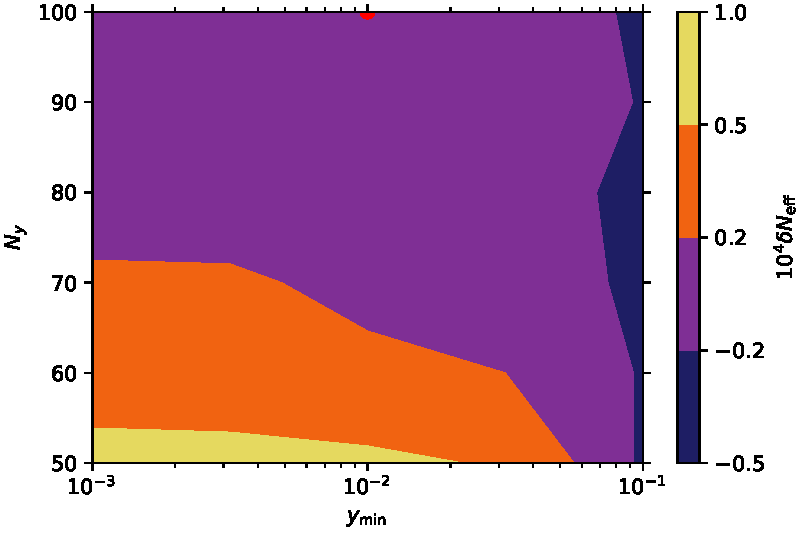
\includegraphics[width=\linewidth]{figures/NC_Ny_ymin.pdf}
\end{subfigure}
\begin{subfigure}{.49\textwidth}
\centering
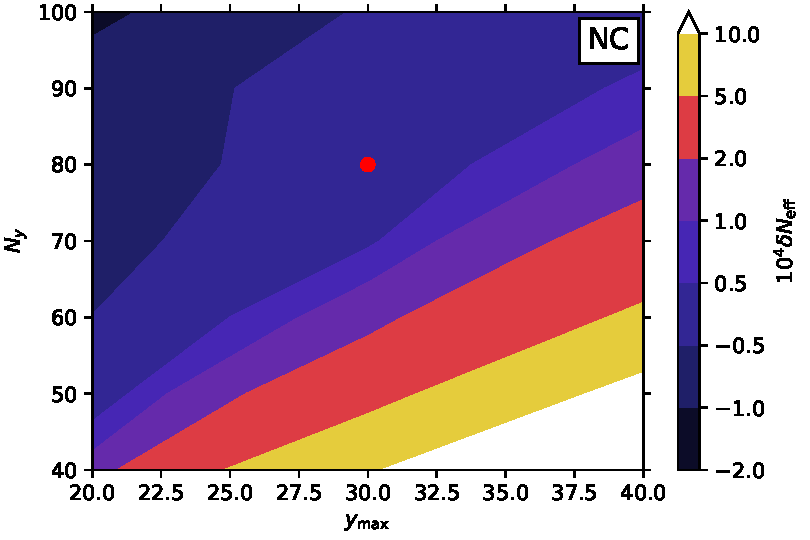
\includegraphics[width=\linewidth]{figures/NC_Ny_ymax.pdf}
\end{subfigure}
\end{center}
\caption{Change in $\Neff^{\rm SM}$ from a full calculation using the Newton--Cotes quadrature method and including the full neutrino--neutrino collision integral,
with respect to variations in the number of $y$-nodes and their range.
{\it Left}: Variations in $N_y$ and~$y_{\rm min}$.
{\it Right}: Variations in $N_y$ and~$y_{\rm max}$.
The default setting of $y_{\rm min}=0.01$, $y_{\rm max}=20$, and $N_y = 100$ is marked by a red dot on each plot.
From \cite{Bennett:2020zkv}.
\label{fig:Ny_yrange}
}
\end{figure}

As a summary, a reasonable estimate of the theoretical and numerical uncertainty on the recommended value
obtained considering three active neutrinos,
$\Neff=3.0433$,
is of order $2\times10^{-4}$ \cite{Bennett:2020zkv}.


\section{Default parameters}
\label{ssec:default}
The numerical constants in the code (defined in \texttt{sources/const.f90})
are mostly taken from the Particle Data Group~\cite{Tanabashi:2018oca,Zyla:2020zbs}.
The default configuration of the code (\texttt{ini/explanatory.ini}) is the following:
\begin{itemize}
\item
\textbf{Neutrino parameters}: three active neutrinos (\texttt{flavorNumber = 3}), with mixing parameters:
\texttt{givesinsq = T} (the following parameters \texttt{thetaij} provide the value of $\sin^2\theta_{ij}$),
\texttt{theta12 = 0.297},
\texttt{theta13 = 0.0215},
\texttt{theta23 = 0.425},
\texttt{dm21 = 7.37e-05} (eV$^2$),
\texttt{dm31 = 0.00256} (eV$^2$).
%
\item
\textbf{Collision integrals}: non-zero (\texttt{collint\_diagonal\_zero = F}) diagonal terms
computed taking into account only the contribution from neutrino--electron interactions
(\texttt{collint\_d\_no\_nue = F}, \texttt{collint\_d\_no\_nunu = T}),
off-diagonal terms computed using damping approximations
(\texttt{collint\_offdiag\_damping = T})
from Eqs.~\eqref{eq:damping_d_r}--\eqref{eq:fittingfunctiondy} (\texttt{collint\_damping\_type = 1}),
also in this case considering only the neutrino--electron interactions
(\texttt{collint\_od\_no\_nue = F}, \texttt{collint\_od\_no\_nunu = T}).
%
\item
\textbf{FTQED}:
finite temperature corrections are enabled
(\texttt{ftqed\_temperature\_corr = T}),
using third order corrections (\texttt{ftqed\_ord3 = T})
but no logarithmic ones (\texttt{ftqed\_log\_term = F}),
and including corrections to the electron mass in the matter potentials
(\texttt{ftqed\_e\_mth\_leptondens = T}).
%
\item
\textbf{Grid settings}:
the $x$ range is considered between
\texttt{x\_in = 0.05} and
\texttt{x\_fin = 35},
and the quantities saved in \texttt{Nx = 500} bins.
For the momentum grid, the default configuration considers \texttt{Ny = 30} momentum nodes
spaced according to the Gauss--Laguerre method (\texttt{use\_gauss\_laguerre = T}),
as neutrino--neutrino collision terms are disabled.
Remember that a correct run with neutrino--neutrino collisions is better performed
using a much denser momentum grid, that will require to disable the Gauss--Laguerre nodes selection.
%
\item
\textbf{Output settings}:
the default output folder is \texttt{outputFolder = output},
checkpoint are active (\texttt{checkpoint = T}),
if a \texttt{resume.dat} file is present in the output folder it will be removed and the run repeated
(\texttt{force\_replace = T}),
all the outputs are enabled (%
\texttt{save\_energy\_entropy\_evolution = T},
\texttt{save\_fd = T},
\texttt{save\_Neff = T},
\texttt{save\_nuDens\_evolution = T},
\texttt{save\_w\_evolution = T},
\texttt{save\_z\_evolution = T}%
).
%
\item \textbf{Precision}:
\texttt{dlsoda\_rtol = 1.d-6},
\texttt{dlsoda\_atol\_z = 1.d-6},
\texttt{dlsoda\_atol\_d = 1.d-6},
\texttt{dlsoda\_atol\_o = 1.d-6}.
\end{itemize}
For more available parameters and the description of all of them, see \texttt{ini/explanatory.ini}.


\section{Precompiler options}
\label{ssec:precompiler}
The compilation of \fortepiano\ may be performed including a number of precompiler options
that alter the behaviour of the code.
The advantage of precompiler options is that the related features are enabled or disabled
before the code is compiled, and their existence in the source code
does not affect the execution speed when they are disabled.

Available precompiler options currently include:
\begin{itemize}
\item \texttt{GLR\_ZERO\_MOMENTUM}: use $g_L$, $\tilde g_L$ and $g_R$ values
computed at zero momentum transfer \cite{Erler:2013xha} in Eq.~\eqref{eq:gLR}.
\item \texttt{FULL\_F\_AB}: full matrix multiplication
when computing neutrino--electron collision integrals
(Eqs.~\eqref{eq:F_ab_sc} and \eqref{eq:F_ab_ann}).
No effect on the code execution unless the diagonal matrices $G_{L,R}$ are modified to be off-diagonal.
\item \texttt{FULL\_F\_NU}: take into account the full neutrino density matrix
when computing neutrino--neutrino collision integrals
(Eqs.~\eqref{eq:F_nunu} and \eqref{eq:F_nubarnu}).
By default, the code only considers the diagonal elements of the neutrino density matrix,
as off-diagonal ones are typically much smaller.
\item \texttt{NO\_INTERPOLATION}: do not interpolate electron/muon energy densities and FTQED corrections
(enabled by default to save time). Incompatible with the use of logarithmic FTQED corrections.
\item \texttt{NO\_MUONS}: disable muon contributions to total energy density and matter potentials.
\item \texttt{NO\_NUE\_ANNIHILATION}: disable contribution from $\nu\bar\nu\leftrightarrow e^+e^-$ processes to collision integrals.
\item \texttt{TESTSPEED}: compute a speed test with a timing of the first 1000 derivatives.
\end{itemize}



\acknowledgments
We thank J.J.~Bennett and G.~Buldgen for helping spotting
some issue in the treatment of finite temperature corrections
and for support in implementing the higher order correction terms,
and M.~Escudero~Abenza for useful comments and suggestions.

This software is part of a project that has received funding from the European Union's Horizon 2020 research and innovation programme, under the Marie Sk{\l}odowska Curie grant agreements No
796941 (ENCORE, until March 2020) and
754496 (FELLINI, starting October 2020).


\bibliographystyle{JHEP}
\bibliography{main}


\end{document}
